\chapter{Appearance Computations}
\label{chap:appearance}

So far, we've covered the fundamental basics of the light and the rendering process to be able to comprehend the more advanced techniques practiced in the computer graphics. As we've mentioned before, our primary goal is to evaluate the computational accuracy of several specific appearance sensations. Even though they are quite common in every day life, their integration to the modern renderers is, to this date, rare.  In this chapter, we discuss these phenomena individually --- their manifestations in the nature, the physics behind them and finally, their computations in the rendering process. 

\section{Polarization}
\label{sec:polarization}



\section{Reflectance}

The reflective surfaces are a surprisingly common sighting. As the perfectly diffuse materials basically do not exist in the nature, a large set of the materials that surround us are considered glossy. In \autoref{sec:BRDF}, we defined a bidirectional reflectance distribution function that defines the reflective properties of a material. 

\subsection{Fresnel}

It is necessary to know the basics of the geometry optics to be able to properly define a reflectance model. First of all, the \emph{Snell's law}~\cite{pharr2016physically}

\begin{equation}
\eta_i sin\theta_i = \eta_t sin\theta_t 
\end{equation}

states that the incoming angle $\theta_i$ (angle between the surface normal and the incoming direction) times the \emph{index of refraction} of the entering medium $\eta_i$ must be equal to their transmitted counterparts. In other words, knowing the indices of refraction of the entering and the leaving media and the incoming direction, we can compute the transmitted direction.

The index of refraction (IOR) varies from material to material (e.g. IOR of glass is \~1.5) and it essentially states how fast the light travels through the specific material.

However, this gives us only the direction of the refracted light. In most cases, we also need to know the ratio between the reflected and the refracted light. Depending on the polarization of the light (further explained in \autoref{sec:polarization}), the \emph{Fresnel equations} take the two following forms~\cite{pharr2016physically}:

\begin{align*}
r_s = \frac{\eta_t cos\theta_i - \eta_i cos\theta_t}{\eta_t cos\theta_i + \eta_i cos\theta_t}\\
r_p = \frac{\eta_i cos\theta_i - \eta_t cos\theta_t}{\eta_i cos\theta_i + \eta_t cos\theta_t} 
\end{align*}

From these, we can compute the \emph{Fresnel reflectance} for an unpolarized light:
\begin{equation}
F_r=\frac{1}{2}(r_s^2 + r_p^2)
\end{equation}

The transmitted energy is equal to $1-F_R$ due to the energy conservation law.

Note that the previous computations describe only a subset of the materials called the \emph{dielectrics}, which are the materials that do not conduct electricity and are capable of transmitting light, such as glass, water, diamond, etc. The second large group consists of the \emph{conductors} which are basically all metals/materials with opaque surfaces. The light is actually transmitted into the conductor, however, due to its physical properties, it is quickly absorbed. There exists a third group of the \emph{semiconductors} which are very rarely considered in the physically based rendering, therefore we skip them. A comparison between a dielectric and a conductor is shown in \autoref{fig:compare_dielectric_conductor}.

\begin{figure}[httpb]
	\centering
	\begin{tabular}{cc}
		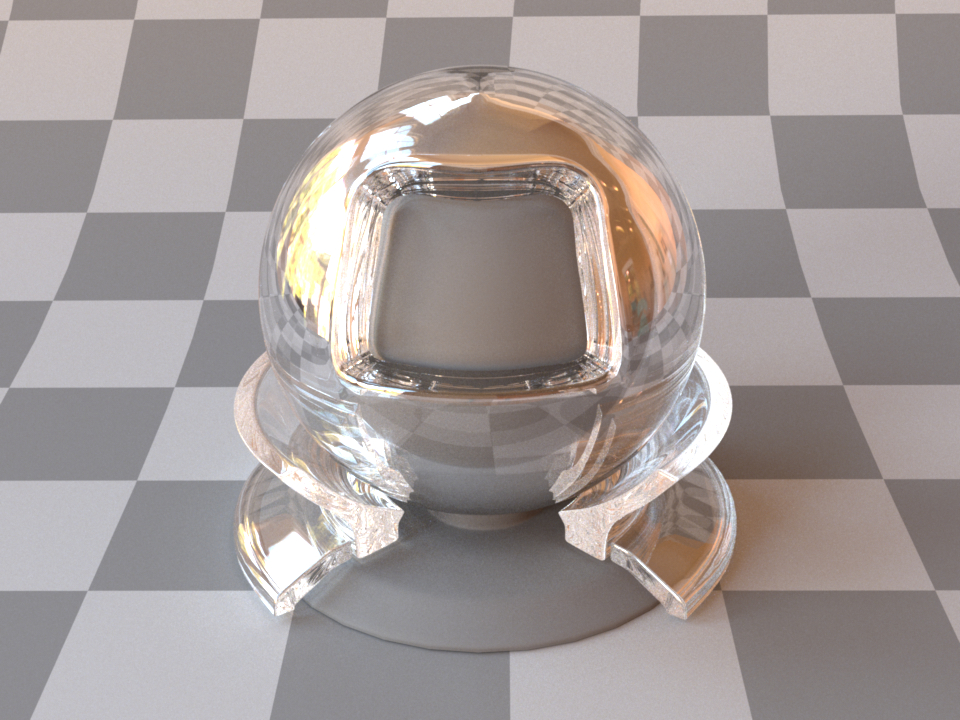
\includegraphics[width=.4\linewidth]{img/dielectric_diamond.jpg}
		&
		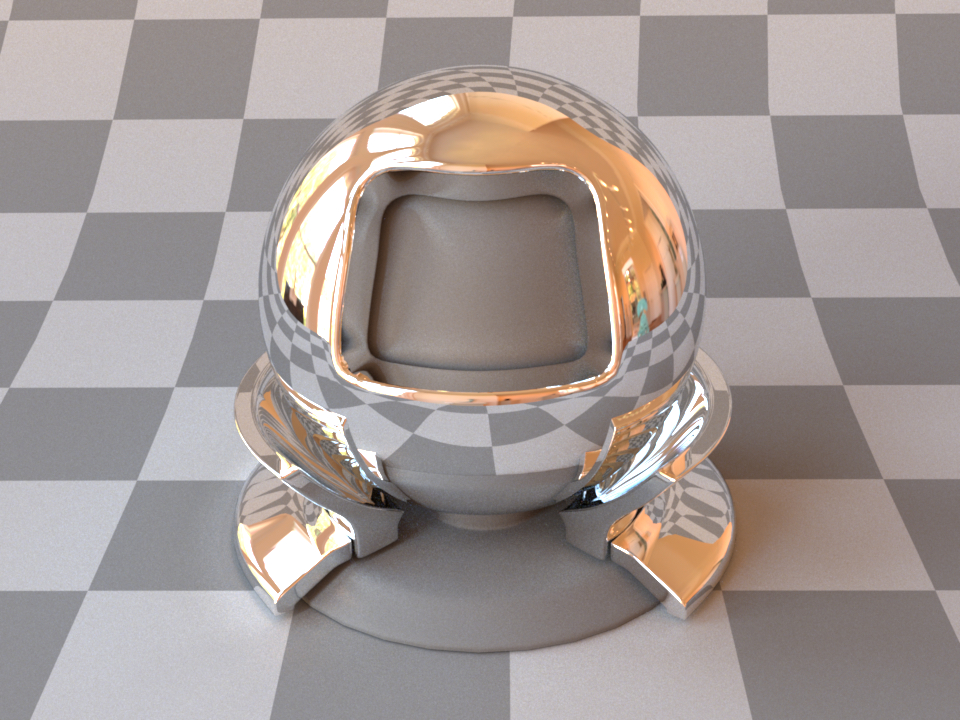
\includegraphics[width=.4\linewidth]{img/conductor_aluminium.jpg}
	\end{tabular}
	\caption{A preview of a dielectric (diamond, left) a  conductor (aluminium, right) rendered in Mitsuba2~\cite{mitsubaWeb}}
	\label{fig:compare_dielectric_conductor}
\end{figure}

While this is a matter of simply computing the Fresnel equations, the practice is more complicated as most of the commonly seen materials are not perfectly smooth. Slight imperfections, either on purpose or due to the manufacturing errors, can be found on a large majority of all materials which makes them rough.

\subsection{Microfacet theory}
With that in mind, the \emph{microfacet theory} was developed by \citet{cook1982reflectance} to address this aspect and provide a theoretical representation of the rough surfaces.

The main idea is that a rough surface consists of the \emph{microfacets} -- a collection of very small surfaces distributed statistically throughout the whole underlying \emph{macrosurface}. We compute the illumination (BRDF) for each of these microfacets (commonly considered to be a perfect mirror) and their aggregate behavior states the final scattering. An example of such distribution is shown in \autoref{fig:microfacets}.

\begin{figure}[httpb]
	\centering
	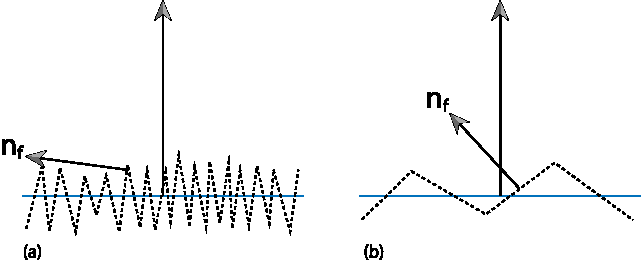
\includegraphics[width=.8\linewidth]{img/microfacets.pdf}
	\caption{A demonstration of a very rough (left) and a relatively smooth (right) microfacet distribution~\cite{pharr2016physically}}
	\label{fig:microfacets}
\end{figure}

As these microfacet computations are local, we need to consider the possibility that they might obscure each other. Three main aspects are accounted for:
\begin{description}
	\item[Masking] Microfacet is not visible from the viewer
	\item[Shadowing] Microfacet is not reachable from the light source
	\item[Interrecflection] Bounces between the microfacets
\end{description}

Many variations to the Cook-Torrance model have been developed, such as it's predecessor Torrance-Sparrow~\cite{Torrance1967TheoryFO} or Oren-Nayar~\cite{oren1994generalization} for diffuse reflectance.

In this thesis, we focus on the distribution functions of the microfacets as they are ultimately the deciding factor of the rough surface look. A nice comparison of the three commonly used microfacet distributions --- \emph{Phong}, \emph{Beckmann} and \emph{GGX} -- along with their distribution functions, masking functions and sampling equations can be found in the \citet{walter2007microfacet}. As the exact formulations of those three methods are not a necessity for this thesis, we provide only a brief overview for each of them and an illustrative comparison between the GGX and the Beckmann of the same roughness in 
\autoref{fig:ggx_beckmann}.

\paragraph{Phong}

Even though the Phong distribution is purely empirical (not physically based), it is still quite popular choice for the microfacet distribution as it is simple to implement and provides sufficient results.

\paragraph{Beckmann}

The Beckmann distribution~\cite{beckmann1987scattering} is already physically based and for a long time has been considered the best solution to the rough surfaces as it is based on the Gaussian roughness. However, with the parameters set appropriately, it still provides the results very similar to the Phong distribution.

\paragraph{GGX}

The GGX distribution~\cite{walter2007microfacet} was introduced as an improvement over the Beckmann's solution for some cases. It maintains stronger tails, thus better shadowing and is based on the measured data of the real rough materials.

\begin{figure}[httpb]
	\centering
	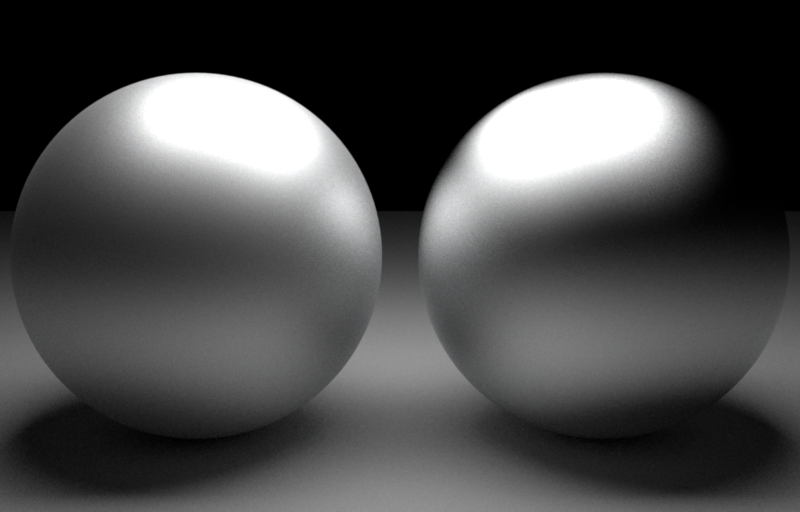
\includegraphics[width=.8\linewidth]{img/ggx_beckmann.png}
	\caption{A rough aluminium sphere with the GGX distribution (left) compared to it's Beckmann equivalent (right) rendered  in Mitsuba2}
	\label{fig:ggx_beckmann}
\end{figure}

\section{Dispersion}

\section{Iridescence}


\section{Fluorescence}